\documentclass[authoryearcitations]{UoYCSproject}

\usepackage{tikz}
\usetikzlibrary{arrows,positioning}

\usepackage{amsmath}

\author{Joshua Asch}

\title{Tracing and Debugging in GP2}

\date{Date TBC}
\supervisor{Detlef Plump}
\MEng
\wordcount{0}


\abstract{
    This is my project!
}


\begin{document}

\maketitle
\listoffigures
\listoftables

\cleardoublepage

\chapter{Introduction}
\label{cha:Introduction}

\section{Introductiony Bit}
\label{sec:IntroductionyBit}

A section introducing the project.

\section{Ethics}
\label{sec:Ethics}

A section discussing the ethics of the project.



\clearpage

\chapter{Literature Review}
\label{cha:LiteratureReview}

%//////////////////////////////////////////////////////////////////////////////

\section{Programming by Graph Transformation}
\label{sec:ProgrammingByGraphTransformation}

%==============================================================================

\subsection{Graph Programming}
\label{sec:GraphProgramming}

Graph programming involves a series of transformations applied to a graph. The
problem being solved must be redefined in terms of a start graph and an algorithm
represented by graph transformations. The final graph at the end of the algorithm
gives the solution to the problem.

Historically, programming by graph transformation required using a programming
language such as C or Java, implementing data structures to represent graphs, and
directly making modifications to the graph in the program. However, recently some
attempts have been made to create tools for graph programming which abstract away
the representation of the graphs, allowing the programmer to focus on the program itself.

Some of these tools include PROGRES \citep{schurr1999}, AGG \citep{ermel1999},
GROOVE \citep{rensink2004}, and, most recently, GP2 \citep{bak2015}. All of these
are domain-specific languages for graph programming which also provide a graphical
interface to describe graphs and transformations.

These kinds of tools take a representation of a graph program, as defined in their
graphical editor, and transform this into a runnable program. This can be implemented
in Java (in the case of AGG and GROOVE) or in C (in the case of PROGRES and GP2). This
program can then be executed to find the output graph generated by the algorithm.

%==============================================================================

\subsection{The GP2 Language}
\label{sec:TheGP2Language}

GP2 is a programming language developed at the University of York \citep{bak2015},
an updated implementation of the original language, GP \citep{plump2009}. It is
designed for writing programs at a high level, to perform graph transformations 
without having to implement data structures to represent the graphs in more
traditional lower level languages such as C.

Programming in GP2 consists of an input graph, known as the \emph{host graph}, a
set of \emph{rules}, and a \emph{program} which defines the order in which to
apply the rules. Running a GP2 program on a host graph produces a new graph as
a result, called the \emph{output graph}.

\subsubsection{Rules}
\label{sec:Rules}

Rules are the basic building blocks of a GP2 program and are defined by a
left-hand-side (LHS), a right-hand-side (RHS), and optionally a conditional
clause. A rule can be thought of as the definition of a transformation; a subgraph
matching the LHS of the rule is transformed to resemble the RHS. An example of a
GP2 rule is shown in \autoref{fig:RuleInGP2}.

\begin{figure}
    \begin{center}
        \begin{tabular}{l}

            \texttt{link}

            \\\\

            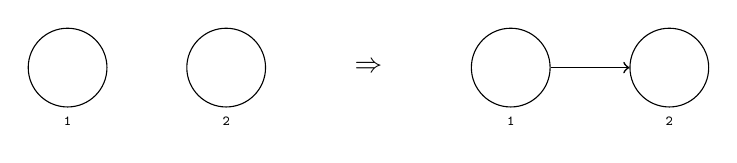
\begin{tikzpicture}
                [vertex/.style={circle,draw,minimum size=10mm},
                 post/.style={<-,semithick}]

                \node         (transition) {$\Rightarrow$}                                {};

                \node[vertex] (lhs 2) [label=below:\tiny{\texttt{2}},left=of transition]  {};
                \node[vertex] (lhs 1) [label=below:\tiny{\texttt{1}},left=of lhs 2]       {};

                \node[vertex] (rhs 1) [label=below:\tiny{\texttt{1}},right=of transition] {};
                \node[vertex] (rhs 2) [label=below:\tiny{\texttt{2}},right=of rhs 1]      {}
                    edge[post] (rhs 1);

            \end{tikzpicture}

            \\

            \texttt{where not edge(1, 2)}

        \end{tabular}
    \end{center}
    \caption{A rule in GP2}
    \label{fig:RuleInGP2}
\end{figure}

The conditional clause is used to specify additional constraints on the subgraph
matching the LHS. Any match has to both match the LHS and conform to the constraints
defined by the conditional clause.

In a compiled program, a rule is split into two phases. The \emph{match} phase
searches the current graph for a subgraph which matches the LHS of the rule. If
a match is found, the program moves on to the second phase, the \emph{application}.
To ensure consistent output between successive program executions, rule matches are
chosen deterministically by the compiled program. If no match is found for the LHS,
the rule is considered \emph{failed}.

During the application phase, any nodes and edges present in the LHS but not the RHS
will be deleted, and any nodes and edges present in the RHS but not the LHS will be
created. At the end of the application phase, the subgraph will match the RHS of the
rule definition. The new graph created by the application of this rule, an \emph{intermediate
graph}, is then used as the input to the next part of the program.

In the example in \autoref{fig:RuleInGP2}, the program will search for a subgraph
containing two nodes without an edge connecting them. If a match is found, it will
be transformed to resemble the RHS by adding an edge between the nodes.

\subsubsection{Programs}

A GP2 program defines the order in which to apply rules using 8 simple control
structures:

\begin{description}
    \item[\textsc{Sequence}]
    Two subprograms separated by a semicolon ``\texttt{P; Q}'' are applied
    one after the other.

    \item[\textsc{Rule Set}]
    Subprograms in curly braces ``\texttt{\{P, Q, R\}}'' define a set, where
    exactly one subprogram from the set is executed, unless no subprograms in
    the set can be matched. The subprogram to execute is chosen deterministically.

    \item[\textsc{If-Then-Else}]
    In the statement ``\texttt{if C then P else Q}'', the sub-program \texttt{C}
    is executed, and the result, i.e. success or failure, is recorded, before
    reverting any changes caused by C. Then, if C succeeded, \texttt{P} is
    executed on the original graph. If it failed, then \texttt{Q} is executed on
    the original graph. Note that by taking a copy first, any changes made by
    \texttt{C} are reverted before executing either \texttt{P} or \texttt{Q}.

    \item[\textsc{Try-Then-Else}]
    Similar to \textsc{If-Then-Else}, but \texttt{C} is only reverted if it fails.
    Thus any changes made by \texttt{C} are \emph{not} reverted before executing
    \texttt{P}, but they \emph{are} reverted before executing \texttt{Q}.

    \item[\textsc{As-Long-As-Possible}]
    A subprogram followed by an exclamation point ``\texttt{P!}'' is matched and
    applied repeatedly until it cannot be matched any more. The final attempt to
    match the LHS will \emph{not} consider the rule \emph{failed}.

    \item[\textsc{Procedure}]
    Similar to a C preprocessor macro, a procedure is simply a named subprogram
    where any reference to the procedure name can be replaced with the definition
    of the procedure.

    \item[\textsc{Skip}]
    A no-op which always succeeds, and does not affect the graph. Invoked using the
    keyword ``\texttt{skip}''.

    \item[\textsc{Fail}]
    A no-op which always fails and does not affect the graph. This is the same as
    attempting to execute a rule for which there are no matches. Invoked using
    the keyword ``\texttt{fail}''.
\end{description}

For GP2, a subprogram is either a single rule, referenced by its name, or one of
the above control structures. Therefore it is possible to nest control structures
to create more complex programs.

In general, execution of a program continues until either all statements are
executed, or until a statement results in an attempt to apply a rule which has
no matches in the graph. The exceptions to this are \textsc{As-Long-As-Possible}
statements, and the conditional statements in \textsc{If-Then-Else} and
\textsc{Try-Then-Else} structures. In these cases, a failure to match a rule
does not halt execution of the program.

%//////////////////////////////////////////////////////////////////////////////

\section{Program Tracing}
\label{sec:ProgramTracing}

%==============================================================================

\subsection{Tracing in Imperative Languages}
\label{sec:TracingInImperativeLanguages}

A section discussing what tracing and debugging imperative languages like C and
Java is like.

%==============================================================================

\subsection{Tracing in Functional Languages}
\label{sec:TracingInFunctionalLanguages}

A section discussing what tracing functional languages like Haskell is like. A
main focus on the Hat tool for Haskell, describing how it relates to the
problem of tracing GP2.

%==============================================================================

\subsection{Previous Work on Tracing GP2}
\label{sec:PreviousWorkOnTracingGP2}

A section discussing the previous project \citep{taylor2016} on this topic.



\clearpage

\chapter{Another chapter...}



\clearpage

\bibliography{references}

\end{document}
